% To je predloga za poročila o domačih nalogah pri predmetih, katerih
% nosilec je Blaž Zupan. Seveda lahko tudi dodaš kakšen nov, zanimiv
% in uporaben element, ki ga v tej predlogi (še) ni. Več o LaTeX-u izveš na
% spletu, na primer na http://tobi.oetiker.ch/lshort/lshort.pdf.
%
% To predlogo lahko spremeniš v PDF dokument s pomočjo programa
% pdflatex, ki je del standardne instalacije LaTeX programov.

\documentclass[a4paper,11pt]{article}
\usepackage{amsmath, amsthm, amssymb}
\usepackage{a4wide}
\usepackage{fullpage}
\usepackage[utf8x]{inputenc}
\usepackage[slovene]{babel}
\selectlanguage{slovene}
\usepackage[toc,page]{appendix}
\usepackage[pdftex]{graphicx} % za slike
\usepackage{setspace}
\usepackage{color}
\definecolor{light-gray}{gray}{0.95}
\usepackage{hyperref}
\renewcommand{\baselinestretch}{1.2} % za boljšo berljivost večji razmak
\renewcommand{\appendixpagename}{Priloge}

\usepackage{listings} % za vključevanje kode
% nastavitve za izpis kode
\lstset{ 
	language=Python,
	basicstyle=\footnotesize,
	basicstyle=\ttfamily\footnotesize\setstretch{1},
	backgroundcolor=\color{light-gray},
}

\title{2. domača naloga: Informativnost značilk\\pri napovedovanju posameznih tem}
\author{Miha Zidar (63060317)}
\date{\today}

\newcommand\q[1]{``#1''}

% dodatni paketi
\usepackage{float}
\graphicspath{{src/}} 
\DeclareGraphicsExtensions{.pdf,.png,.jpg,.jpeg}

\begin{document}
\maketitle

\section{Uvod}

V tej nalogi smo si pogledali odvisnost razredov in atributov. Za"celi smo z diskretizacijo vseh vrednosti na 2 dela: elementi ve"cji od 0 in elementi enaki 0. Nato smo se za vsak par atributov z pomo"cjo permutacijskega testa odlo"cili ali obstaja dovolj zanesljiva povezava med vrednostjo atributa in vrednostjo razreda. 

\section{Metode}
\subsection{Infomacijski prispevek}
Za ocenjevanje kakovosti atributov smo uporabili mero infomacijski prispevek (information gain) med atributom in razredom. 

\subsubsection*{Definicija}
Enačba za izračun informacijskega prispevka je:
\[\mbox{Gain}(Y,X)\ =\ \mbox{H}(Y) - \mbox{H}(Y|X)\ =\ \mbox{I}(Y,X)\]

\[\mbox{I}(Y,X)\ =\ \sum_{y\in Y}\ \sum_{x\in X} p(x,y) \log \Bigg(\frac{p(x,y)}{p(x)*p(y)}\Bigg) \]

\subsubsection*{Primer}
Podani imamo dve naklju"cni spremenljivki, ki v na"si nalogi predstavljata dva stolplca v tabeli. $X$ predstavlja na"s stolpec pod atributom, $Y$ pa vrednosti v na"sem razredu.
\[
 \begin{matrix}
  X & = & (0,0,1,0,0,1) \\
  Y & = & (0,1,1,0,0,1)
 \end{matrix}
\]
Sedaj izra"cunamo vse potrebne verjetnosti.
\[
\begin{tabular}{rcl}
  p(X=0) & = & 4/6 \\
  p(X=1) & = & 2/6 \\
  p(Y=0) & = & 3/6 \\
  p(Y=1) & = & 3/6 \\
  p(X=0,Y=0) & = & 3/6 \\
  p(X=0,Y=1) & = & 1/6 \\
  p(X=1,Y=0) & = & 0/6 \\
  p(X=1,Y=1) & = & 2/6 \\
\end{tabular} 
\]
Vstavimo te verjetnosti v zgornjo ena"cbo in dobimo:
\[ 3/6 \log \Bigg(\frac{3/6}{(4/6)*(3/6)}\Bigg)\ +\ 1/6 \log \Bigg(\frac{1/6}{(4/6)*(3/6)}\Bigg)\ +\ 0 \ +\ 2/6 \log \Bigg(\frac{2/6}{(2/6)*(3/6)}\Bigg)\]
Ko "stevila vnesmo v octave, nam izpise rezultat (kjer aX predstavlja posamezni "clen ena"cbe):
\begin{verbatim}
octave:19> a1+a2+a3+a4
ans =  0.459147917027245
\end{verbatim}
moj program pa za "stevili $9$ ($0b1001$) in $25$ ($0b11001$) vrne $0.459147917027$, kar je enako vendar z nekaj decimalnimi mesti manj. Za razliko od Orange orodja ki pa se v povpre"cju razlikuje "ze na sedmem decimalnem mestu, kar sem tudi preveril z dodatnim testnim programom ki je ra"cunal povpre"cno odstopanje od mojih izra"cunanih vrednosti.

\subsection{Permutacijski test}

Prmutacijski test en izmed na"cinov kako ugotovimo ali je informacijski prispevek na"sega atributa za podani razred dober, ali pa je tak le zaradi naklju"cja. To pa ugotovimo enostavno tako, da primerjamo informacijski prispevek na"sega razreda z mnogimi naklju"cnimi permutacijami tega razreda. Na koncu se odlo"cimo o pomembnosti atributa glede na to, koliko procentov naklju"cnih permutacij je pokazalo vi"sji informacijski prispevek. Tej stopnji zaupanja bomo rekli $alpha$ in spodaj imamo prikazano "stevilo pomembnih atributov, ki jih dobimo pri razli"cnih vrednosti $alpha$.\\

\subsection{Program in optimizacija}

Ker smo ra"cunali z dosti podatki, smo pri"sli do "casovnega problema, in sicer navaden permutacijski test za 100 permutacij je trajal priblizno 2h. Iz optimizacijskih razlogov sem se zato odlo"cil da ne uporabljam orange, vendar hranim podatke na druga"cen na"cin in sam ra"cunam informacijski prispevek za te podatke. Tako sem "cas izvajanja zmanj"sal iz 2h na priblizno 3 minute. \\

Ker imamo opravka le z binarnimi atributi, nima smisla vsakega elementa hraniti v seznamu, vendar je prostorsko in procesorsko dosti bolj u"cinkovito "ce posamezne stolpce predstavimo kot navadna "stevila. V taki predstavitvi pa imamo "se eno prednost: za "stetje kje so enake ali razli"cne vrednosti lahko uporabljamo enostavne bitne operacije, ki so mnogo hitrej"se kot operacije nad seznami.\\

Ko pa imamo podatke lepo predstavljene, pa potrebujemo "se nekaj extra podatkov, ker se za"cetne nule pri "stevilih druga"ce izgubijo. Tako sem za vsako "stevilo hranil koliko je dolgo, koliko enic vsebuje in stevilo samo. Napisal pa sem tudi vse potrebne funkcije za delovanje, Kar si lahko pogledate v kodi.



\section{Rezultati}

Za prikaz rezultatov smo pognali permutacijski test z 500 permutacijami, in re"sitev predstavili z histogramom ki prikazuje koliko pomembnih atributov imamo pri razlicnih alpha vrednostih. Histogram bi sicer dosti lepse zgledal ce bi bil urejen po entropiji posameznega razreda, vendar mi tega "se ni uspelo dokon"cati, saj so podatki lo"ceni med seboj, kar mi je povzro"calo te"zave. V rezultatih pa vidimo kako hitro raste stevilo pomembnih atributov v odvisnosti od alpha, saj ko je alpha $0.1$ so pri nekaterih razredih pomembni skoraj vsi atributi. 
\begin{figure}[H]
\begin{center}
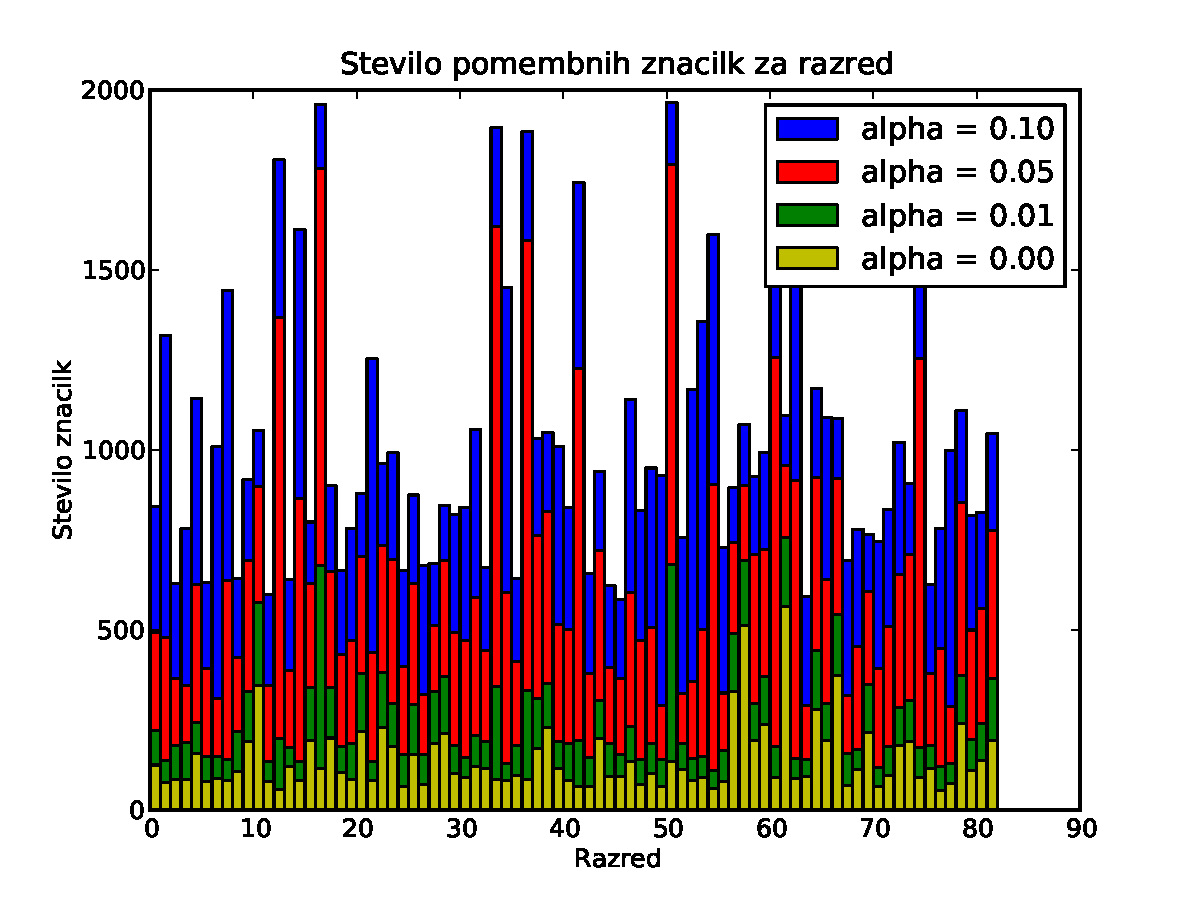
\includegraphics[scale=0.6]{muraw.pdf}
\caption{Prikaz stevila pomembnih atributov za posamezne razrede, pri razlicnih alpha vrednostih.}
\label{slika1}
\end{center}
\end{figure}

Ena stvar, ki sem jo opazil je, da lahko pri zelo majhni spremembi v kodi (naprimer pogoj za gledanje ali je razred pomemben zamenjamo iz $<=$ na $<$) lahko dobimo zelo velike spremembe v rezultatih (v enem primeru je stevilo znacilk padlo iz 300 na 50). Zato sem izrisal "se histogram ki prikazuje porazdelitev posameznih vrednosti izra"cunanega informacijskega prispevka pri 2000 permutacijah. Rezultat je bil zelo nepricakovan, vendar je lepo pojasnil velika odstopanja v majhni spremembi pogoja.

\begin{figure}[H]
\begin{center}
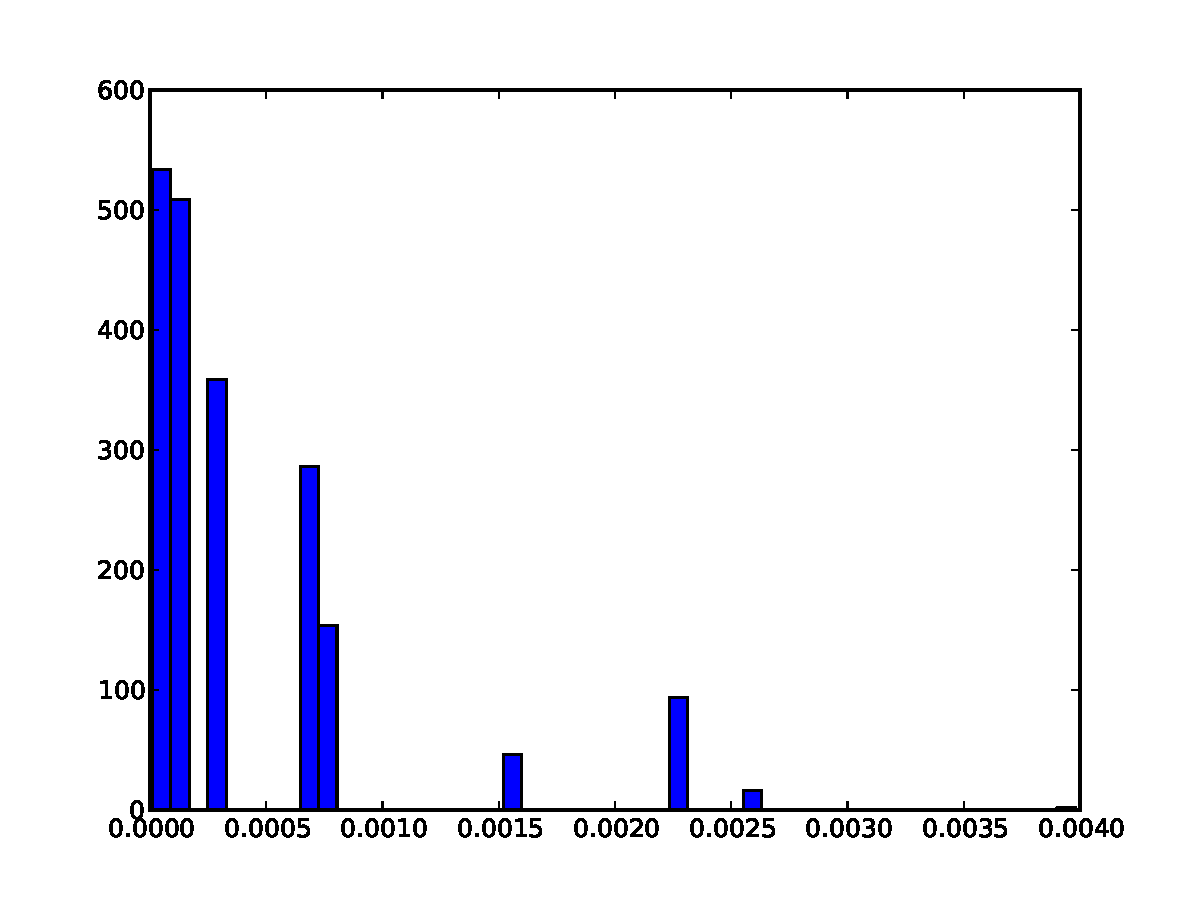
\includegraphics[scale=0.4]{testc40D_1404Orange.pdf}
\caption{porazdelitev info gain za razred c40 pri atributu D\_1404, za 2000 permutacij.}
\label{slika1}
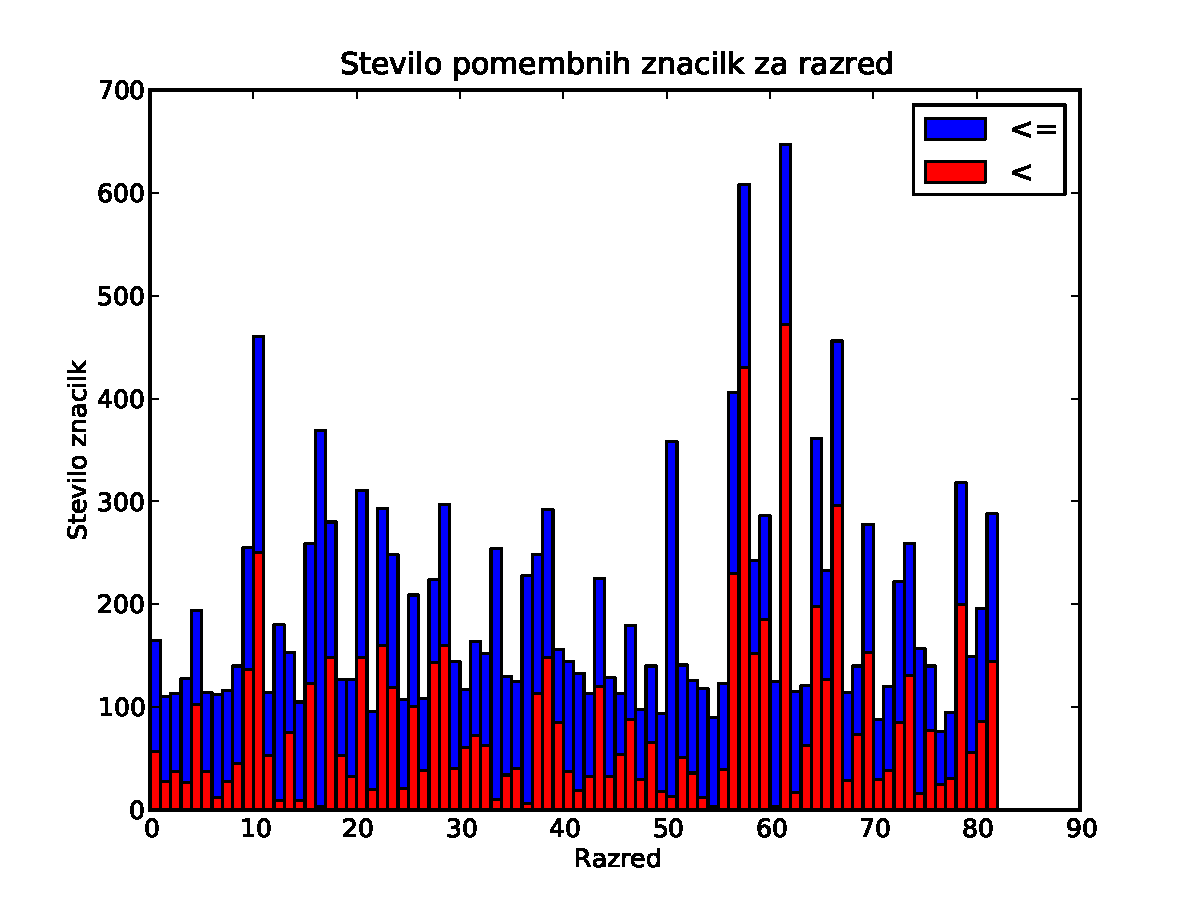
\includegraphics[scale=0.4]{muraawdva.pdf}
\caption{Odstopanje stevila zna"cilk za posamezni razredi pri pogojih $<=$ na $<$ za izlo"canje, ter pri $alpha=0$.}
\label{slika1}
\end{center}
\end{figure}\ \\[-40pt]

Izka"ze se, da je velikokrat dosti enakih vrednosti, kar vidimo "ze iz nizke entropije atributov. Iz tega sklepam da bi bilo bolj smiselno te rezultate primerjati "se z kak"sno drugo mero za ocenjevanje atributov enkrat v prihodnosti, zaenkrat pa so te rezultati "cisto zadovoljivi.


\section{Izjava o izdelavi domače naloge}
Domačo nalogo in pripadajoče programe sem izdelal sam.


\end{document}
